%% LyX 2.4.0~beta5 created this file.  For more info, see https://www.lyx.org/.
%% Do not edit unless you really know what you are doing.
\documentclass[english]{foils}
\usepackage[T1]{fontenc}
\usepackage[latin9]{inputenc}
\pagestyle{foilheadings}
\setcounter{secnumdepth}{1}
\setcounter{tocdepth}{1}
\usepackage{xcolor}
\usepackage{url}
\usepackage{amsmath}
\usepackage{amsthm}
\usepackage{amssymb}
\usepackage{graphicx}

\makeatletter

%%%%%%%%%%%%%%%%%%%%%%%%%%%%%% LyX specific LaTeX commands.
%% A simple dot to overcome graphicx limitations
\newcommand{\lyxdot}{.}


%%%%%%%%%%%%%%%%%%%%%%%%%%%%%% Textclass specific LaTeX commands.
\theoremstyle{definition}
\newtheorem{defn}{\protect\definitionname}

%%%%%%%%%%%%%%%%%%%%%%%%%%%%%% User specified LaTeX commands.
\usepackage{xcolor}
\renewcommand{\labelitemi}{$\textcolor{blue}{\bullet}$}
\renewcommand{\labelitemii}{$\textcolor{teal}{\Rightarrow}$}
\renewcommand{\labelitemiii}{$\textcolor{red}{\rightarrow}$}
\renewcommand{\labelitemiv}{$\textcolor{brown}{\circ}$}
% for French theorems, etc. since I'm using English to fix bullet pb.
\providecommand{\examplename}{Example}
\providecommand{\definitionname}{Definition}
\providecommand{\theoremnname}{Theorem}
\providecommand{\remarkname}{Remark}
\providecommand{\exercisename}{Exercise}
% DT book stuff
\newcommand{\argmin}{\operatornamewithlimits{argmin}} % for a "clean" argmin 
\newcommand{\T}{\mathrm{T}}  % transpose
\newcommand{\PP}{\mathrm{P}}  % probability
\newcommand{\dd}{\mathrm{d}} % integration dx
\newcommand{\ee}{\mathrm{e}} % exponential
\newcommand{\E}{\mathrm{E}} % expectation
%_%_%_%_%_%_%_%_
% for tikz drawings and cartoons
%_%_%_%_%_%_%_%_

\usepackage{tikz}

% for tikzit drawings
\usepackage{tikzit}
\input{flow.tikzstyles}


% for decision trees:
\tikzset{
	treenode/.style = {shape=rectangle, rounded corners,
		draw, align=center,
		top color=white, bottom color=blue!20},
	root/.style     = {treenode, font=\Large, bottom color=red!30},
	env0/.style     = {treenode, font=\large, bottom color=orange!30},
	env1/.style     = {treenode,  bottom color=green!30},
	env/.style      = {treenode, font=\ttfamily\normalsize},
    leaf/.style      = {treenode, font=\ttfamily\normalsize},
	dummy/.style    = {circle,draw}
}
\usetikzlibrary{positioning}

%_%_%_%_%_%_%_%_%_%_
% for algorithms and listings
%_%_%_%_%_%_%_%_%_%_

%\usepackage{algorithm_MA,algpseudocode}
%\usepackage{algorithmic}
\usepackage{algpseudocode}

%\floatstyle{ruled}
%\newfloat{algorithm}{tbp}
%\providecommand{\algorithmname}{Algorithm}
%\floatname{algorithm}{\protect\algorithmname}
%

% try and fix \Comment problem due to excessive defs in Chap. DA
\algrenewcommand{\algorithmiccomment}[1]{%
	\hfill$\triangleright$\ \textcolor{darkgray}{#1}}

\usepackage{tcolorbox}

\makeatother

\usepackage{babel}
\providecommand{\definitionname}{Definition}

\begin{document}

\MyLogo{SciML: Ethics and Bias}
\title{SciML - Trustworthiness, Ethics and Bias}
\author{Mark Asch - IMU/VLP/CSU }
\date{2023}
\maketitle

\foilhead{Program}
\begin{enumerate}
\item Ethics and responsible use of scientific machine learning:
\begin{enumerate}
\item Inference Cycle
\item SSL and LLMs
\item Bias in machine learning models.
\item Fairness in machine learning.
\item Transparency in machine learning.
\item Trustworthiness, explainability.
\item The ethical challenges of using scientific machine learning.
\item The responsible use of scientific machine learning.
\end{enumerate}
\end{enumerate}

\foilhead{Some sayings...}
\begin{quotation}
\textcolor{teal}{ML sucks. LLMs suck. {[}LeCun 2023{]}}
\end{quotation}
\bigskip{}

\begin{quotation}
\textcolor{teal}{Weapons of Math Destruction}
\end{quotation}
\bigskip{}

\begin{quotation}
\textcolor{teal}{Algorithms are not rascist. }

\textcolor{teal}{Your skin is just too} dark.
\end{quotation}

\foilhead{$\;$}

\vfill{}

\begin{center}
{\Large\textbf{\textcolor{blue}{THE INFERENCE CYCLE}}}{\Large\par}
\par\end{center}

\vfill{}


\foilhead{SciML and Digital Twins}
\begin{itemize}
\item We begin with a quote {[}K. Willcox, 2019{]}
\end{itemize}
\begin{quote}
\textcolor{teal}{Learning from data through the lens of models is
a way to bring structure to an otherwise intractable problem: it is
a way to respect physical constraints, to embed domain knowledge,
to bring interpretability to results, and to endow the resulting predictions
with quantified uncertainties.}
\end{quote}
\begin{itemize}
\item One possible definition of a \textcolor{magenta}{Digital Twin }is
the following {[}AIAA, 2020{]}
\end{itemize}
\begin{defn}
[Digital Twin]A Digital Twin is a set of virtual information constructs
that mimics the structure, context and behavior of an individual/unique
physical asset, or a group of physical assets, is dynamically updated
with data from its physical twin throughout its life cycle and informs
decisions that realize value., if
\end{defn}

\foilhead{SciML and Digital Twins - pragmatic}
\begin{itemize}
\item In a more pragmatic way, If we take into account: 
\begin{itemize}
\item The availability of (large) volumes of (often real-time) data. 
\item The accessibility to this data. 
\item The tools and implementations of ML/AI-based algorithms. 
\item The body of knowledge of mathematical models. 
\item The readiness and low cost of computational devices. 
\end{itemize}
\item Then we have all the necessary ingredients for creating a \textcolor{magenta}{virtual
counterpart }of a physical object or system. 
\item This\textbf{\textcolor{red}{{} ``digital twin''}} can then accompany
its physical counterpart, possibly throughout the object's \textcolor{magenta}{life
cycle}. 
\item In fact, recent developments in machine learning, could enable \textcolor{magenta}{auto-repair}
and reprogramming of the twin as it ingests more and more data, and
learns more and more about the physical plant. 
\item The twin then includes both \textcolor{magenta}{static} and \textcolor{magenta}{dynamic}
parts. 
\begin{itemize}
\item The static part consists of the initial model, process and design
specifications. 
\item The dynamic part includes the simulation process, coupled with data
acquisition, and finally auto-updating.
\end{itemize}
\end{itemize}

\foilhead{The Inference Cycle}
\begin{center}
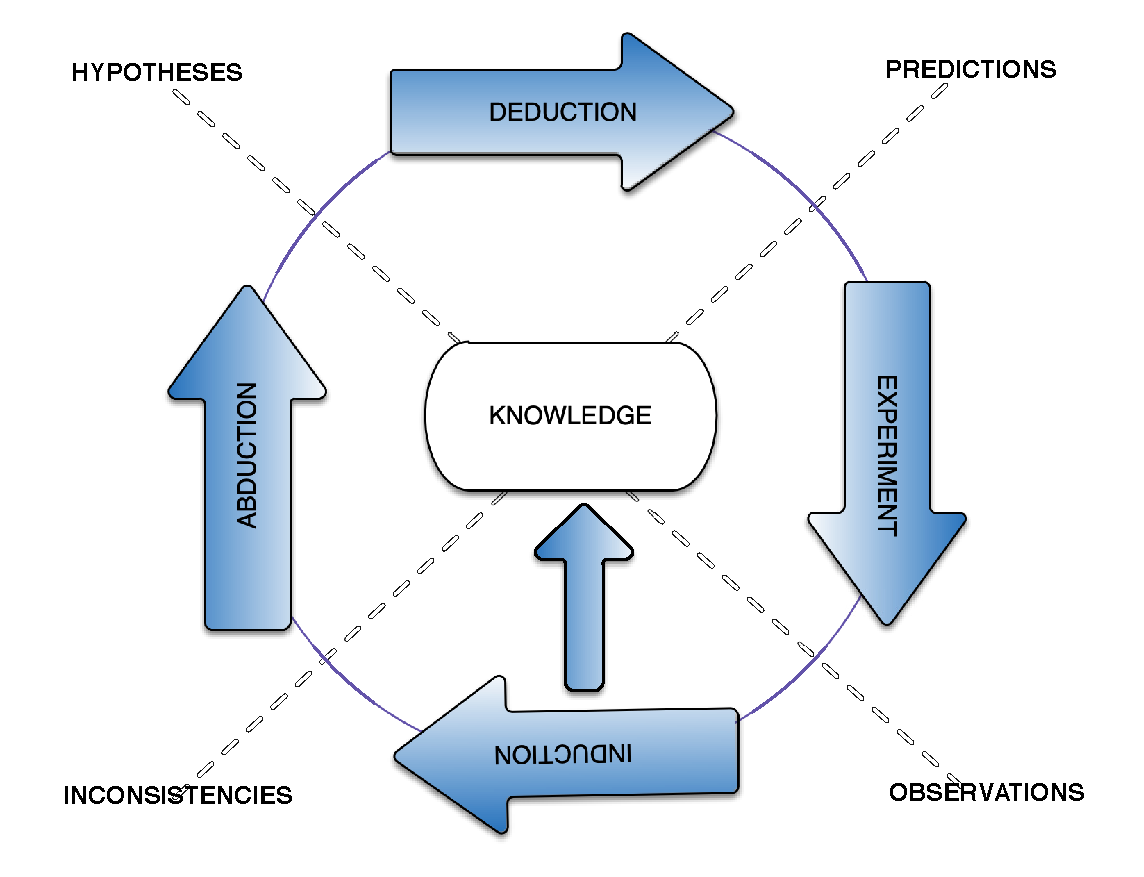
\includegraphics[width=0.8\textwidth]{graphics/InfCycle0}
\par\end{center}
\begin{itemize}
\item How can we conceptualize the approach to digital twins and SciML? 
\begin{itemize}
\item A broader view will be indispensable because, as will be illustrated
in the numerous examples, a digital twin based on SciML is a complex
object that combines 
\begin{itemize}
\item modeling, 
\item simulation, 
\item optimization, 
\item machine learning, 
\item uncertainty quantification, etc. 
\end{itemize}
\item So, it is important to see where we are, and where we are going.
\end{itemize}
\item The inference cycle provides this global vision. The above Figure
presents the key \textcolor{magenta}{logical elements} of the \textcolor{magenta}{scientific
process}. 
\begin{itemize}
\item It expresses the classic view that the scientific method is a complex\textcolor{magenta}{{}
inferential process} that seeks to improve our predictive understanding
of nature by building on a foundation of thorough and carefully controlled
observation. 
\end{itemize}
\end{itemize}

\foilhead[-0.5in]{The Inference Cycle - 3 forms of Inference}
\begin{center}
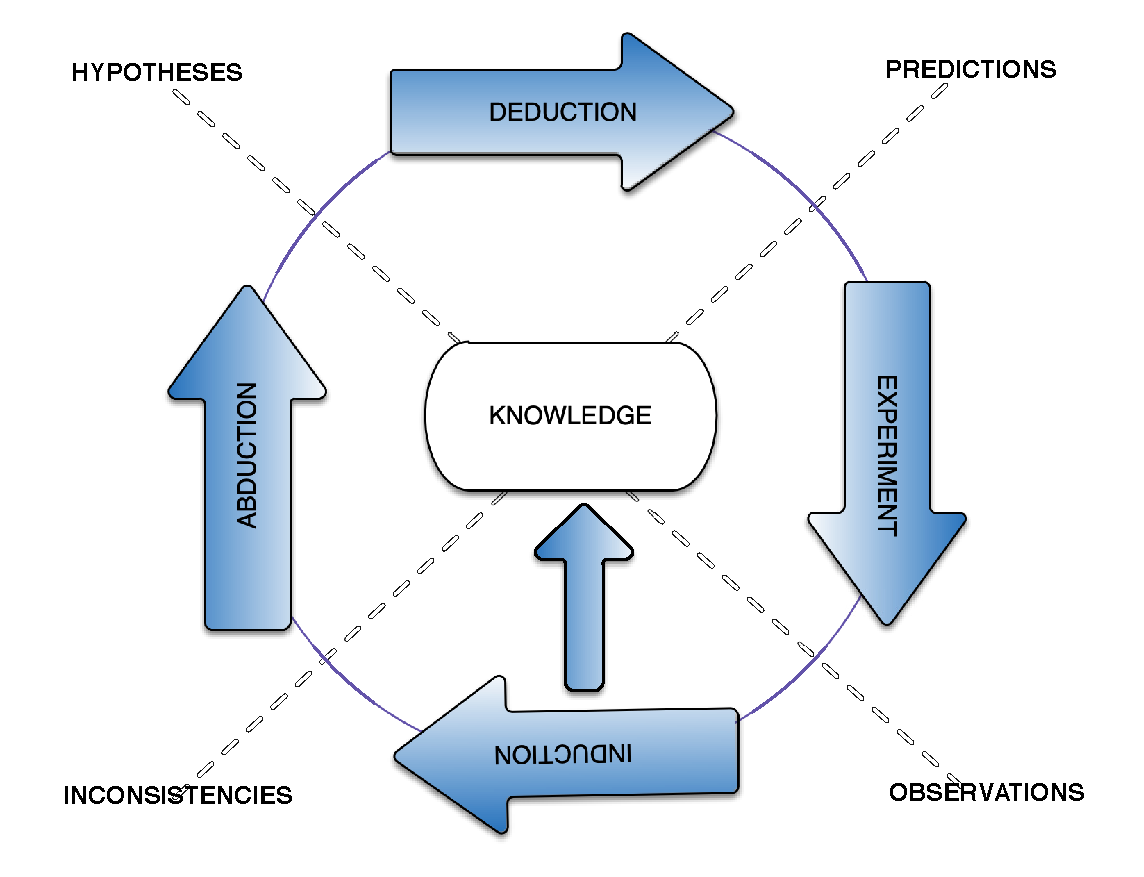
\includegraphics[width=0.45\textwidth]{graphics/InfCycle0}
\par\end{center}
\begin{enumerate}
\item \textbf{Abduction}---going from (unexplained) effect to (possible)
cause, i.e., guessing at an \textcolor{magenta}{explanation}. 
\item \textbf{Deduction}---going from cause to effect, i.e., drawing out
the necessary \textcolor{magenta}{consequences} of a set of propositions. 
\item \textbf{Induction}---going from specific to general, i.e., making
a sampling-based \textcolor{magenta}{generalization}. This is the
process of evaluation, where we either accept the model and increase
our state of belief, or we identify a mismatch, or inconsistency and
we need to find a new hypothesis (by abduction) to test in the next
deductive-inductive phase. 
\end{enumerate}

\foilhead{The Inference Cycle - Lessons}
\begin{itemize}
\item We must not confuse abduction with deduction. 
\begin{itemize}
\item That is, if your (deductive stage) model produces a result, you cannot
assume that this is the truth. 
\item The truth has to be tested, then reprocessed through the induction
stage, before \textcolor{magenta}{updating your belief}---nothing
more.
\end{itemize}
\item Knowledge is only a \textcolor{magenta}{state of belief}---what we
\emph{believe} to be right, to the best of our actual knowledge. 
\begin{itemize}
\item That is why the cycle does not really end, we keep on going round
and round, improving our state of belief at each cycle (see Figure).
\end{itemize}
\item The inference cycle acts as a \textcolor{magenta}{compass}, not telling
us how to get there, but rather where we are, where to go and what
the next step should be. 
\item The cycle can be \textcolor{magenta}{enriched} with all the possible
methods enabling the passage from phase to phase. 
\begin{itemize}
\item At the highest level, these are computational modeling and data analysis,
or machine learning. 
\item At the next level, we have to dig into the toolbox and extract the
right methods from within these two. 
\item Overall, we will probably/ideally need to mix and match, employing
tools from both.
\end{itemize}
\end{itemize}

\foilhead[-0.5in]{The Inference Cycle - Quotes}
\begin{itemize}
\item From {[}Flach, Kakas, Ray 2006{]}
\end{itemize}
\begin{quote}
\textcolor{teal}{Modeling a scientific domain is a continuous process
of observing and understanding phenomena according to some currently
available model, and using this understanding to improve the original
domain model. In this process one starts with a relatively simple
model which gets further improved and expanded as the process is iterated.
At any given stage of its development, the current model is very likely
to be incomplete. The task then is to use the information given to
us by experimental observations to improve and possibly complete this
description. The development of our theories is driven by the observations
and the need for these theories to conform to the observations. This
point of view forms the basis of many formal theories of scientific
discovery (see Popper, Kuhn) in the sense that the development of
a scientific theory is considered to be an }\textcolor{orange}{incremental
process of refinement strongly guided by the empirical observations}\textcolor{teal}{.}
\end{quote}
\begin{itemize}
\item From {[}Peirce, Collected Papers, 1978{]}
\end{itemize}
\begin{quote}
\textcolor{teal}{141. All positive reasoning is of the nature of judging
the proportion of something in a whole collection by the proportion
found in a sample. Accordingly, there are three things to which we
can never hope to attain by reasoning, namely, }\textcolor{orange}{absolute
certainty, absolute exactitude, absolute universality.}\textcolor{teal}{{}
We cannot be absolutely certain that our conclusions are even approximately
true; for the sample may be utterly unlike the unsampled part of the
collection. We cannot pretend to be even probably exact; because the
sample consists of but a finite number of instances and only admits
special values of the proportion sought. Finally, even if we could
ascertain with absolute certainty and exactness that the ratio of
sinful men to all men was as 1 to 1; still among the infinite generations
of men there would be room for any finite number of sinless men without
violating the proportion. The case is the same with a seven legged
calf.}
\end{quote}
\bigskip{}

\begin{quote}
\textcolor{teal}{142. Now if exactitude, certitude, and universality
are not to be attained by reasoning, there is certainly }\textcolor{orange}{no
other means }\textcolor{teal}{by which they can be reached. }
\end{quote}

\foilhead{The Robot Scientist}
\begin{itemize}
\item More formally, 
\begin{itemize}
\item given a \textcolor{magenta}{theory} $T$ describing our current (incomplete)
model of the scientific domain under investigation, and 
\item a set of \textcolor{magenta}{observations} $O,$ 
\item \textcolor{magenta}{\emph{abduction}} and \textcolor{magenta}{\emph{induction}}
are employed in the process of incorporating the new information contained
in the observations $O,$ into the current theory $T.$ 
\item They both synthesize new knowledge, $H,$ that extends the current
model to $T\cup H$ such that the union is \textcolor{magenta}{consistent}
and obtained by using the \emph{deductive} process.
\end{itemize}
\item The concept of a ``Robot Scientist'' {[}King 2009{]} was used to
test the \textcolor{red}{automation} of this\textcolor{magenta}{{} abductive
reasoning}, where a hypothesis $H$ is generated to explain a goal
$G$ with respect to a theory $T.$ This is actually a form of Machine
Learning, in its purest sense. 
\item The robot proceeds by:
\begin{itemize}
\item hypothesizing to explain observations, 
\item devising experiments to test these hypotheses, 
\item physically running the experiments using laboratory robotics, 
\item interpreting the results from the experiments, 
\item repeating the cycle as required. 
\end{itemize}
\item This sounds familiar---just replace the robot by a human research
engineer trying to build a DT using SciML, and we are in the inference
cycle of scientific research.
\item \textcolor{magenta}{Bayesian Optimization} can be used to help in
the choice of optimal parmeters for the nect cycle.
\end{itemize}

\foilhead{$\;$}

\vfill{}

\begin{center}
{\Large\textbf{\textcolor{blue}{SSL and LLMs - the future?}}}{\Large\par}
\par\end{center}

\vfill{}


\foilhead{Self-Supervised Learning (SSL) and Large Language Models (LLMs) }
\begin{itemize}
\item {[}LeCun, 2023{]}
\begin{itemize}
\item ``ML sucks'' (compared to humans and animals)
\begin{itemize}
\item a 17 year-old can learn to drive a car in 20h of practice, but we
still don't have Level-5 autonomous driving
\end{itemize}
\item Self-Supervised Learning (SSL) (= filling in the blanks) has taken
over the world
\begin{itemize}
\item performance is amazing (``we are fooled by their fluency''), but
they (LLMs) make stupid mistakes
\item they have no common sense and cannot plan their responses 
\item in general, they're very bad at math---but plugins, such as Mathematica,
are changing this
\end{itemize}
\item ``Large Language Models (LLMs) suck''
\begin{itemize}
\item good for: writing assistance (first draft, style polishing), code
writing assistance
\item bad for: producing factual and consistent answers (hallucinations!),
reasoning, planning, math, using tools such as search engines, calculators,
databases
\end{itemize}
\item The world is only partially predictable, so how to deal with this?
\item Solutions: 
\begin{itemize}
\item JEPA (joint embedding architectures), 
\item energy-based models (replace probabilistic models that are intractable)
\item spiked neural networks (closer to brain functions), etc.
\item \textcolor{magenta}{ETHICS} and \textcolor{magenta}{BIAS} analysis
\end{itemize}
\end{itemize}
\end{itemize}

\foilhead{LLM Impacts}
\begin{itemize}
\item Significant impacts already in
\begin{itemize}
\item software productivity
\item basic science and drug design: Alpha-Fold helping to design COVID
vaccines
\item transportation safety
\item healthcare, radiology
\item weather and climate predictions
\end{itemize}
\end{itemize}

\foilhead[-0.5in]{LLMs in the (near) Future}
\begin{itemize}
\item Small number of highly intelligent multimodal LLMs, 10x size of today\textquoteright s 
\item Open source, smaller LLMs that are downloadable and proliferate worldwide 
\item Many specialized LLMs for healthcare, legal work, finance, \ldots{} 
\item LLMs using diverse plugins (calculators, route planners, databases,
LLMs,\ldots ) 
\item Multi-modal models increasingly able to act in the physical world 
\item Personal LLMs for everybody, knowledgeable about each individual user.
\item Wider use in education: how we educate and what we teach.
\end{itemize}
\begin{tcolorbox}[colback=red!5!white,colframe=red!75!black,title=Conclusion] 
LLMs will require extensive norms and controls, in paricular with respect to ethics,  privacy and bias.
\end{tcolorbox}

\foilhead{$\;$}

\vfill{}

\begin{center}
{\Large\textbf{\textcolor{blue}{TRUST AND TRUSTWORTHINESS}}}{\Large\par}
\par\end{center}

\vfill{}


\foilhead{Definitions}

These are current working definitions of key terms, from AI2ES\footnote{\url{https://www.ai2es.org/}}
who are actively working to develop clear, shared definitions of these
terms \cite{BAMS2}.
\begin{description}
\item [{Explainable}] AI---An explainable AI method is one that can be
explained \textcolor{magenta}{post hoc}, after training, in a way
that makes it \textcolor{magenta}{understandable} (Schwalbe and Finzel
2021; Mueller et al. 2021). This includes methods to promote transparency
into the black boxes, such as the ability to measure the importance
of a variable or to see the effect of the values of that variable
on the model as well as methods that allow a user to visualize patterns
of activation in neural networks.
\item [{Interpretable}] AI---An interpretable AI method is a model that
is designed to be \textcolor{magenta}{understood by humans} without
additional explanation. This does not include methods with large numbers
of hyperparameters such as neural networks.
\item [{Interactivity---}] The more interactive a method is, the more
an end user can change parameters, select features, change weights
on data points or parameters, visualize and select a specific model
or ensemble of models, and change how they view the explanation and
AI output (Rudin et al. 2022).
\item [{Trustworthiness}] Trustworthiness and trust are related, yet distinct,
concepts. \textcolor{magenta}{Trust is relational}, in that it is
\textquotedblleft given to\textquotedblright{} or \textquotedblleft placed
in\textquotedblright{} someone or something, and trustworthiness is
evaluative, in that it is a perceived characteristic of someone or
something. With this in mind, trustworthiness is a (potential) trustor\textquoteright s
evaluation, or perception, of whether, when, why, or to what degree
someone or something should or should not be trusted. Current efforts
to develop standards for trustworthiness (e.g., High-Level Expert
Group on AI 2019) may lead some to confuse the broader concept of
perceived trustworthiness with assessment of compliance with formal
standards or policies for trustworthiness. A key distinction is that
\textcolor{magenta}{trustworthiness is a subjective evaluation} that
is largely dependent on the perceptions, values, experiences, and
context of the assessor, which may or may not be influenced by standards
or policies for trustworthiness.
\item [{Deontological---}] Derived from the Greek word for duty (deon).
Deontological ethics are rule-based ethics, or \textcolor{magenta}{moral
duties}, such as the moral duty to be honest (Alexander and Moore
2021).
\item [{AI-Bias---}] AI bias, is a phenomenon that occurs when an algorithm
produces results that are systemically prejudiced due to erroneous
assumptions in the machine learning (ML) process.
\end{description}

\foilhead{Definitions of Trust}
\begin{enumerate}
\item Trust is the willingness of a party to be vulnerable to the actions
of another party based on the expectation that the other will perform
a particular action important to the trustor, irrespective of the
ability to monitor or control that other party. (e.g., Mayer et al
1995) 
\item Trust: In the presence of uncertainty, the degree to which someone
does or does not rely on, or put faith in, someone or something (Wirz
et al.) 
\begin{enumerate}
\item Definition is purposefully broad, so as to capture the many different
definitions and related dimensions of trust. 
\item Our definition of trust is designed to capture trust in all forms. 
\end{enumerate}
\item Trust is the relationship between a trustor and a trustee: the trustor
trusts the trustee. Trust is dynamic, evolves with interactions, and
is easier to lose than gain.
\item \textbf{AI2ES Definition}: Trust is the willingness to assume risk
by relying on or believing in the actions of another party.
\end{enumerate}

\foilhead{Context and Trust}

Trust is invaribaly \textcolor{magenta}{context-dependent}
\begin{description}
\item [{Actors:}] Who is being expected to trust? 
\item [{Targets:}] What are they being expected to trust? 
\item [{Purpose:}] What should they trust something/someone for?
\item [{Reason:}] Why should they trust someone/something? 
\item [{Setting:}] In what place or role are they being asked to trust?
\end{description}

\foilhead{Trustworthiness}
\begin{itemize}
\item \textbf{Aim}: how to develop trustworthy AI/SciML for environmental
sciences?
\begin{itemize}
\item the foundations of trustworthiness for AI 
\item explanatory AI (XAI): how explanations, physics, and robustness can
help build trust in AI 
\item the relationship between ethics and trustworthiness 
\item how machine-learning systems have been developed for a range of environmental
science applications
\end{itemize}
\item XAI offers the opportunity for scientists to 
\begin{itemize}
\item gain insights about the decision strategy of NNs, 
\item help fine tune and optimize models, 
\item gauge trust,
\item investigate new physical insights to establish new science.
\end{itemize}
\item Trustworthy Artificial Intelligence for Environmental Science (TAI4ES)
Summer School
\end{itemize}

\foilhead{Definitions of Trustworthiness}
\begin{itemize}
\item Trust is \textcolor{magenta}{relational} - there is an actor (trustor)
and target (trustee)
\begin{itemize}
\item Who or what am I trusting, and what am I trusting it for? 
\end{itemize}
\item Trustworthiness is \textcolor{magenta}{evaluative} - why should I
trust you?
\item \textbf{AI2ES Definition}: Trustworthiness is a trustor\textquoteright s
evaluation, or perception, of whether, when, why, or to what degree
someone or something should or should not be trusted.
\end{itemize}

\foilhead{$\;$}

\vfill{}

\begin{center}
{\Large\textbf{\textcolor{blue}{ETHICS AND BIAS}}}{\Large\par}
\par\end{center}

\vfill{}


\foilhead{Definitions and Context}
\begin{itemize}
\item \textquotedblleft one reason to desire \textcolor{magenta}{trust}
is an \textquoteleft almost necessary\textquoteright{} condition on
ethical action: that the user has a reasonable belief that the system
(whether human or machine) will behave approximately as intended.\textquotedblright{}
(Danks, AIES\textquoteright 19)
\item Both \textcolor{magenta}{bias} and \textcolor{magenta}{uncertainty}
(including error, or noise) can cause a system to behave in unintended
ways.
\item More broadly, whether an action is \textcolor{magenta}{ethical} may
depend on either the process or the outcomes of the action: 
\begin{itemize}
\item utility/benefits (consequentialism), 
\item whether it is virtuous/the right thing to do (virtue ethics), or 
\item whether it is required by moral principles or duties (deontological
ethics)
\end{itemize}
\item \textcolor{magenta}{Honesty} is a deontological imperative, to respect
others\textquoteright{} rights and dignity, and the autonomy of their
will. \textquotedblleft Be honest\textquotedblright{} is also a virtue
rule.
\end{itemize}

\foilhead{How can AI go wrong in Environmental Sciences?}

Issues related to \textcolor{magenta}{training data}: 
\begin{enumerate}
\item Non-representative training data, including lack of geo-diversity. 
\item Training labels are biased or faulty. 
\item Data is affected by adversaries. 
\end{enumerate}
Issues related to \textcolor{magenta}{AI models}: 
\begin{enumerate}
\item Model training choices. 
\item Algorithm learns faulty strategies. 
\item AI learns to fake something plausible. 
\item AI model used in inappropriate situations. 
\item Non-trustworthy AI model deployed. 
\item Lack of robustness in the AI model. 
\end{enumerate}
Other issues related to \textcolor{magenta}{workforce and society}: 
\begin{enumerate}
\item Globally applicable AI approaches may stymie burgeoning efforts in
developing countries. 
\item Lack of input or consent on data collection and model training.
\item Scientists might feel disenfranchised. 
\item Increase of CO2 emissions due to computing.
\end{enumerate}

\foilhead{Bias}
\begin{itemize}
\item Different types of bias:
\begin{itemize}
\item Computational/Model Bias
\item Data Bias
\item Decision-Making Bias
\item bias-variance tradeoff (recall ML lectures)
\end{itemize}
\item Sources of bias
\begin{itemize}
\item from training data
\item from flawed data sampling
\end{itemize}
\item One of the most complex steps is also the most obvious---understanding
and measuring \textquotedblleft fairness.\textquotedblright{}
\begin{itemize}
\item causality and counterfactual fairness
\end{itemize}
\item fairness vs. bias
\item mitigation strategies and methods
\end{itemize}

\foilhead{Data Bias}
\begin{itemize}
\item The data itself can contain biases, which affect the AI/ML model 
\begin{itemize}
\item Biases could be caused by underlying human biases (e.g. unintentional
or intentional).
\item Biases can be caused by sampling and selection of data. 
\end{itemize}
\item Potential definition: 
\begin{itemize}
\item A class imbalance or distortion in the data from what we know is true,
based on environmental and other knowledge about parameters of interest
\end{itemize}
\end{itemize}

\foilhead{Decision-Making Bias}
\begin{itemize}
\item \textcolor{magenta}{Heuristics} in human decision making 
\begin{itemize}
\item \textcolor{magenta}{Perceptual} biases - motion, color, orientation
(Wolfe, Psych Bull \& Rev 28{[}4{]}, 2021) orientation 
\item \textcolor{magenta}{Memory} biases 
\begin{itemize}
\item working memory (Miller\textquoteright s \textquotedblleft magical
number seven plus or minus two\textquotedblright ) 
\item categorization biases, determined in part by expertise 
\end{itemize}
\item \textcolor{magenta}{Attribute} substitution (Kahneman \& Frederick,
2002), such as 
\begin{itemize}
\item Representativeness heuristic 
\item Affect heuristic 
\end{itemize}
\item \textcolor{magenta}{Anchoring }and adjustment, for example - 
\begin{itemize}
\item familiarity, salience 
\item Example: preference to use models and tools that are familiar to you 
\end{itemize}
\item \textcolor{magenta}{Systemic} biases stemming from social norms and
institutions also affect decision making.
\end{itemize}
\end{itemize}

\foilhead{Ethics and Bias}
\begin{itemize}
\item Ethical Principles can provide a foundation for trustworthy AI, as
illustrated by the European Commission HLEG on AI 2019\footnote{https://digital-strategy.ec.europa.eu/en/library/ethics-guidelines-trustworthy-ai}
\textcolor{magenta}{Ethics Guidelines} for \textcolor{magenta}{Trustworthy
AI}
\end{itemize}
\begin{center}
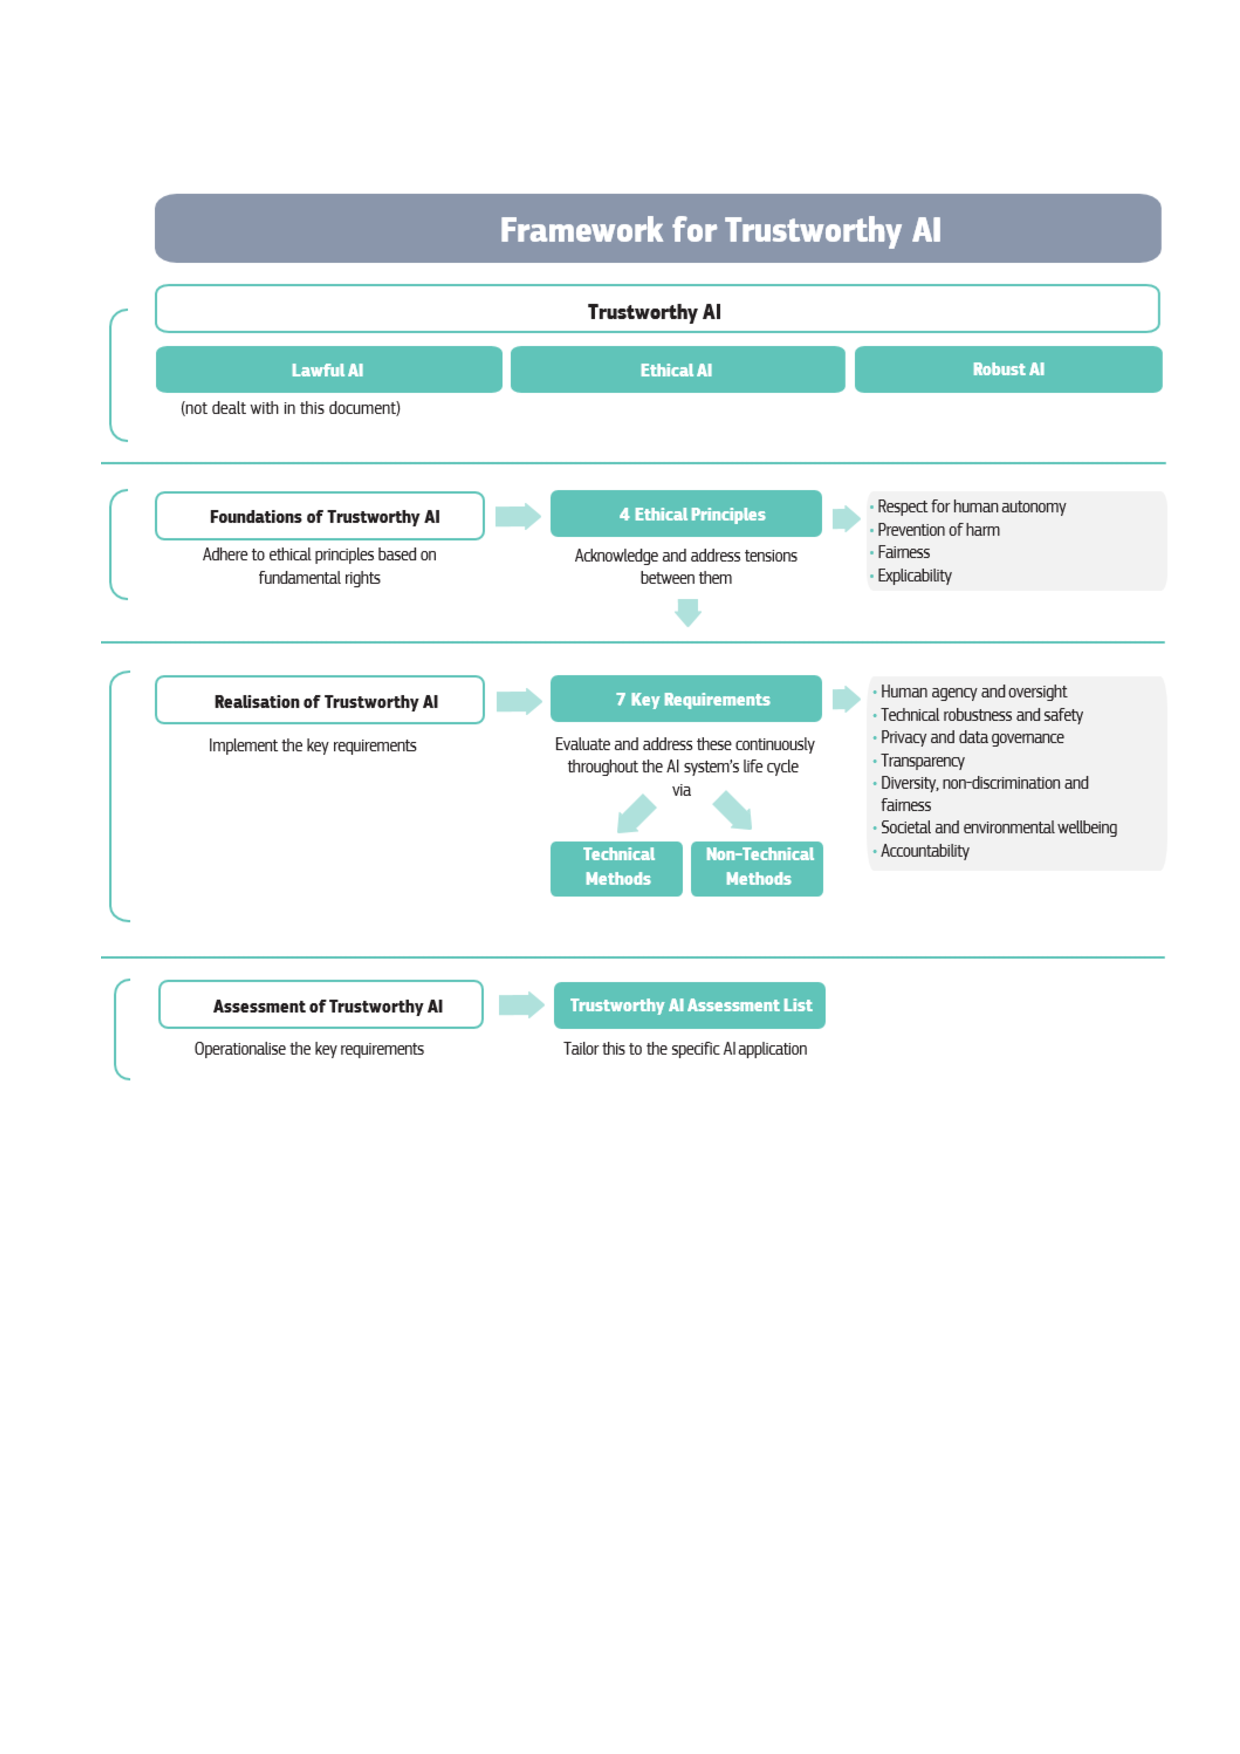
\includegraphics[width=0.9\textwidth]{graphics/ai-ethics-guidelines}
\par\end{center}
\begin{itemize}
\item 4 \textcolor{magenta}{Principles}
\begin{enumerate}
\item Respect for human autonomy
\item Prevention of harm
\item Fairness
\item Explicability
\end{enumerate}
\item 7 Key \textcolor{magenta}{Requirements}
\begin{itemize}
\item \textbf{Human agency and oversight} Including fundamental rights,
human agency and human oversight
\item \textbf{Technical robustness and safety} Including resilience to attack
and security, fall back plan and general safety, accuracy, reliability
and reproducibility
\item \textbf{Privacy and data governance} Including respect for privacy,
quality and integrity of data, and access to data
\item \textbf{Transparency} Including traceability, explainability and communication
\item \textbf{Diversity, non-discrimination and fairness} Including the
avoidance of unfair bias, accessibility and universal design, and
stakeholder participation
\item \textbf{Societal and environmental wellbeing} Including sustainability
and environmental friendliness, social impact, society and democrac
\item \textbf{Accountability }Including auditability, minimisation and reporting
of negative impact, trade-offs and redress.
\end{itemize}
\item Key Guidance for \textcolor{magenta}{Realization} of Trustworthy AI:
\begin{itemize}
\item Ensure that the AI system\textquoteright s entire life cycle meets
the seven key requirements for Trustworthy AI.
\item Consider technical and non-technical methods to ensure the implementation
of those requirements. 
\item Foster research and innovation to help assessing AI systems and to
further the achievement of the requirements; disseminateresults and
open questions to the wider public, and systematically train a new
generation of experts in AI ethics. 
\item Communicate, in a clear and proactive manner, information to stakeholders
about the AI system\textquoteright s capabilities and limitations,
enabling realistic expectation setting, and about the manner in which
the requirements are implemented. Be transparent about the fact that
they are dealing with an AI system. 
\item Facilitate the traceability and auditability of AI systems, particularly
in critical contexts and situations. 
\item Involve stakeholders throughout the AI system\textquoteright s life
cycle. Foster training and education so that all stakeholders are
aware of and trained in Trustworthy AI. 
\item Be mindful that there might be fundamental tensions between different
principles and requirements. Continuously identify, evaluate, document
and communicate these trade-offs and their solutions.
\end{itemize}
\item Key Guidance for \textcolor{magenta}{Assessment} of Trustworthy AI:
\begin{itemize}
\item Adopt a Trustworthy AI assessment list when developing, deploying
or using AI systems, and adapt it to the specific use case in which
the system is being applied. 
\item Keep in mind that such assessment list will never be exhaustive. Ensuring
Trustworthy AI is not about ticking boxes, but about continuously
identifying requirements, evaluating solutions and ensuring improved
outcomes throughout the AI system\textquoteright s lifecycle, and
involving stakeholders therein.
\end{itemize}
\end{itemize}
\begin{tcolorbox}[colback=red!5!white,colframe=red!75!black,title=Conclusion] 
Unethical and biased models should not be trusted!
\end{tcolorbox}

\foilhead{$\;$}

\vfill{}

\begin{center}
{\Large\textbf{\textcolor{blue}{EXPLAINABLE AND INTERPRETABLE}}}{\Large\par}
\par\end{center}

\vfill{}


\foilhead{Explainable AI - Methods}
\begin{itemize}
\item Theoretical topics:
\begin{itemize}
\item the difference between interpretable and explainable AI, 
\item trust vs. trustworthiness, and 
\item model-dependent vs. model-agnostic explanation. 
\end{itemize}
\item Practical explanation methods:
\begin{itemize}
\item the J-measure, 
\item permutation- and impurity-based variable importance, 
\item sequential forward and backward variable selection, 
\item partial-dependence plots, 
\item saliency maps, 
\item class-activation maps, 
\item integrated gradients, 
\item feature visualization,
\item backward optimization, and 
\item novelty detection.
\end{itemize}
\item Finally, augmented explanation methods, which include 
\begin{itemize}
\item physical constraints and 
\item checks for statistical significance.
\end{itemize}
\end{itemize}
\begin{tcolorbox}[colback=red!5!white,colframe=red!75!black,title=Conclusion] 
These require a separate course on Advanced Statistical Methods for model evaluation...
\end{tcolorbox}

\foilhead{Global vs. Local Explainability}
\begin{itemize}
\item \textbf{Global explanations} attempt to describe the model as a whole
\begin{itemize}
\item What are the \textcolor{magenta}{important} \textcolor{magenta}{features}?
\item What \textcolor{magenta}{relationship} has been learned for this feature? 
\end{itemize}
\item \textbf{Local explanations} attempt to describe individual predictions
\begin{itemize}
\item Which feature is making the biggest \textcolor{magenta}{impact} on
the prediction for this example?
\item If this feature value was slightly \textcolor{magenta}{different},
how would it change the prediction?
\end{itemize}
\end{itemize}

\foilhead{Global Explainability}

Global explainability methods can be divided into 3 categories:
\begin{enumerate}
\item Feature \textcolor{magenta}{Importance}/Relevance
\begin{itemize}
\item Importance: How does this feature contribute to the model\textquoteright s
performance?
\item Relevance: How does this feature contribute to the model\textquoteright s
prediction?
\end{itemize}
\item Feature \textcolor{magenta}{Effects}
\begin{itemize}
\item What is the relationship between this feature\textquoteright s values
(or these set of features) and the model\textquoteright s prediction?
\end{itemize}
\item Feature \textcolor{magenta}{Interactions}
\begin{itemize}
\item How is a feature\textquoteright s effect impacted by the effects of
other features?
\end{itemize}
\end{enumerate}

\foilhead{Local Explainability}

The most common local explanation methods are known as \textcolor{magenta}{feature
attribution} methods where we assume that a model\textquoteright s
prediction$P$ can be interpreted as a linear combination of contributions
from each feature
\[
P=\phi_{0}+\sum_{j=1}^{p}\phi_{j},
\]
 where
\begin{itemize}
\item $\phi_{0}$ is the average prediction
\item the second term is the sum of the contributions from each feature
\end{itemize}

\foilhead{Feature Importance}
\begin{itemize}
\item Establishing the important features helps inform the explainability
downstream.
\item Given their greedy nature, ML models will tend to favor only a subset
of the total features they are trained on.
\item Thus, explaining an ML model largely comes down to explaining the
top features. 
\item By knowing the top features we can ask the following questions:
\begin{itemize}
\item How much more \textcolor{magenta}{important} are they than the less
important features?
\item What are the learned \textcolor{magenta}{relationships} for these
top features?
\item What features are \textcolor{magenta}{interacting} with them?
\end{itemize}
\end{itemize}

\foilhead{Other methods}
\begin{itemize}
\item \textcolor{magenta}{Permutation importance}: determine the importance
of a feature by removing it from the model and evaluating how the
model performance suffers. 
\item \textcolor{magenta}{Partial dependence}: evaluate the sensitivity
of a model\textquoteright s prediction to changes in the value for
a particular feature.
\item \textcolor{magenta}{Shapley values:} $\phi_{i}$ for feature $x_{i}$
is the weighted average difference in model prediction when it is
included and not included in some subset of features for all possible
features subsets.
\end{itemize}

\foilhead{$\;$}

\vfill{}

\begin{center}
{\Large\textbf{\textcolor{blue}{INTERPRETABILITY}}}{\Large\par}
\par\end{center}

\vfill{}


\foilhead{Interpretability}
\begin{center}
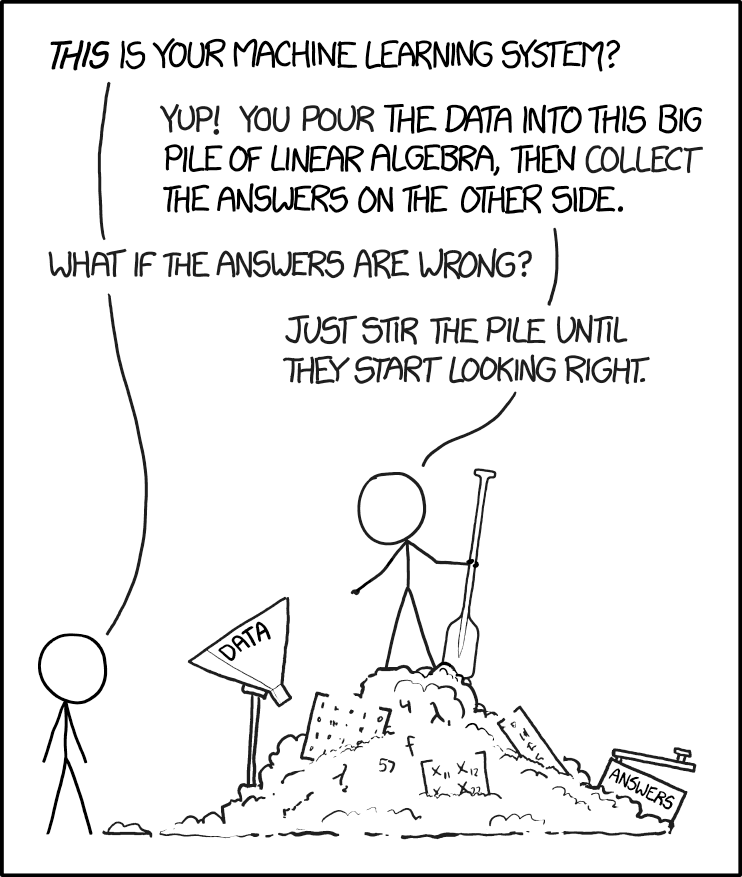
\includegraphics[totalheight=0.6\textheight]{graphics/machine_learning_2x}
\par\end{center}

This is definitely \textcolor{red}{not }the way to go!!!
\begin{itemize}
\item Meaning of interpretabilty
\begin{itemize}
\item dictionary: to explain or to present in understanble terms
\item ML: degree to which a human can understand the cause of a decision
\end{itemize}
\end{itemize}

\foilhead{Interpretability---importance}
\begin{itemize}
\item With widespread use of machine learning (ML), the \textcolor{magenta}{importance}
of interpretability has become clear in avoiding catastrophic consequences. 
\item \textcolor{magenta}{Black box} predictive models, which by definition
are inscrutable, have led to serious societal problems that deeply
affect health, freedom, racial bias, and safety. 
\item \textcolor{magenta}{Interpretable predictive models}, which are constrained
so that their reasoning processes are more understandable to humans,
are much easier to troubleshoot and to use in practice.
\item It is universally agreed that interpretability is a key element of
\textcolor{magenta}{trust} for AI models {[}Rudin 2022{]}
\end{itemize}

\foilhead{Interpretability---black boxes}
\begin{defn}
[Black Box ML Model]A black box machine learning model is a formula
that is either too complicated for any human to understand, or proprietary,
so that one cannot understand its inner workings. 
\end{defn}
\begin{itemize}
\item Black box models are difficult to \textcolor{magenta}{troubleshoot},
which is particularly problematic for medical or health data. 
\item Black box models often predict the right answer for the wrong reason
(the \textquotedblleft Clever Hans\textquotedblright{} phenomenon),
leading to excellent performance in training but \textcolor{magenta}{poor
performance} in practice---this is the brittleness phenomenon related
to the \textcolor{magenta}{bias-variance }trade-off.
\item There are numerous other \textcolor{magenta}{issues} with black box
models. 
\begin{itemize}
\item In criminal justice, individuals may have been subjected to years
of extra prison time due to typographical errors in black box model
inputs. 
\item Poorly-designed proprietary models for air quality have had serious
consequences for public safety during wildfires. 
\item Both of these situations may have been easy to avoid with \textcolor{magenta}{interpretable}
models---see below for further explanations.
\end{itemize}
\item In cases where the underlying distribution of data changes (called
\textcolor{magenta}{domain shift}, which occurs often in practice),
problems arise if users cannot troubleshoot the model in real-time,
which is much harder with black box models than interpretable models. 
\item Standard performance metrics (such as area under the ROC curve --
AUC) can be misconstrued as representing the value of a model in practice,
potentially leading to \textcolor{magenta}{overconfidence} in the
performance of a black box model. Specifically, a reported AUC can
easily be inflated by including many \textquotedblleft obvious\textquotedblright{}
cases in the sample over which it is computed.
\item Determining whether a black box model is \textcolor{magenta}{fair}
with respect to gender, poverty or racial groups is much more difficult
than determining whether an interpretable model has such a bias. 
\item In medicine, black box models turn computer-aided decisions into automated
decisions, precisely because physicians cannot understand the reasoning
processes of black box models. 
\item While interpretable AI is an \textcolor{magenta}{enhancement} of human
decision making, black box AI is a \textcolor{magenta}{replacement}
of it.
\item \textcolor{magenta}{Explaining} black boxes, rather than replacing
them with interpretable models, can make the problem worse by providing
misleading or false characterizations. 
\end{itemize}
\begin{tcolorbox}[colback=red!5!white,colframe=red!75!black,title=Conclusion] 
There is a clear need for innovative machine learning models that are inherently interpretable.
\end{tcolorbox}

\foilhead{Knowledge Discovery Process}

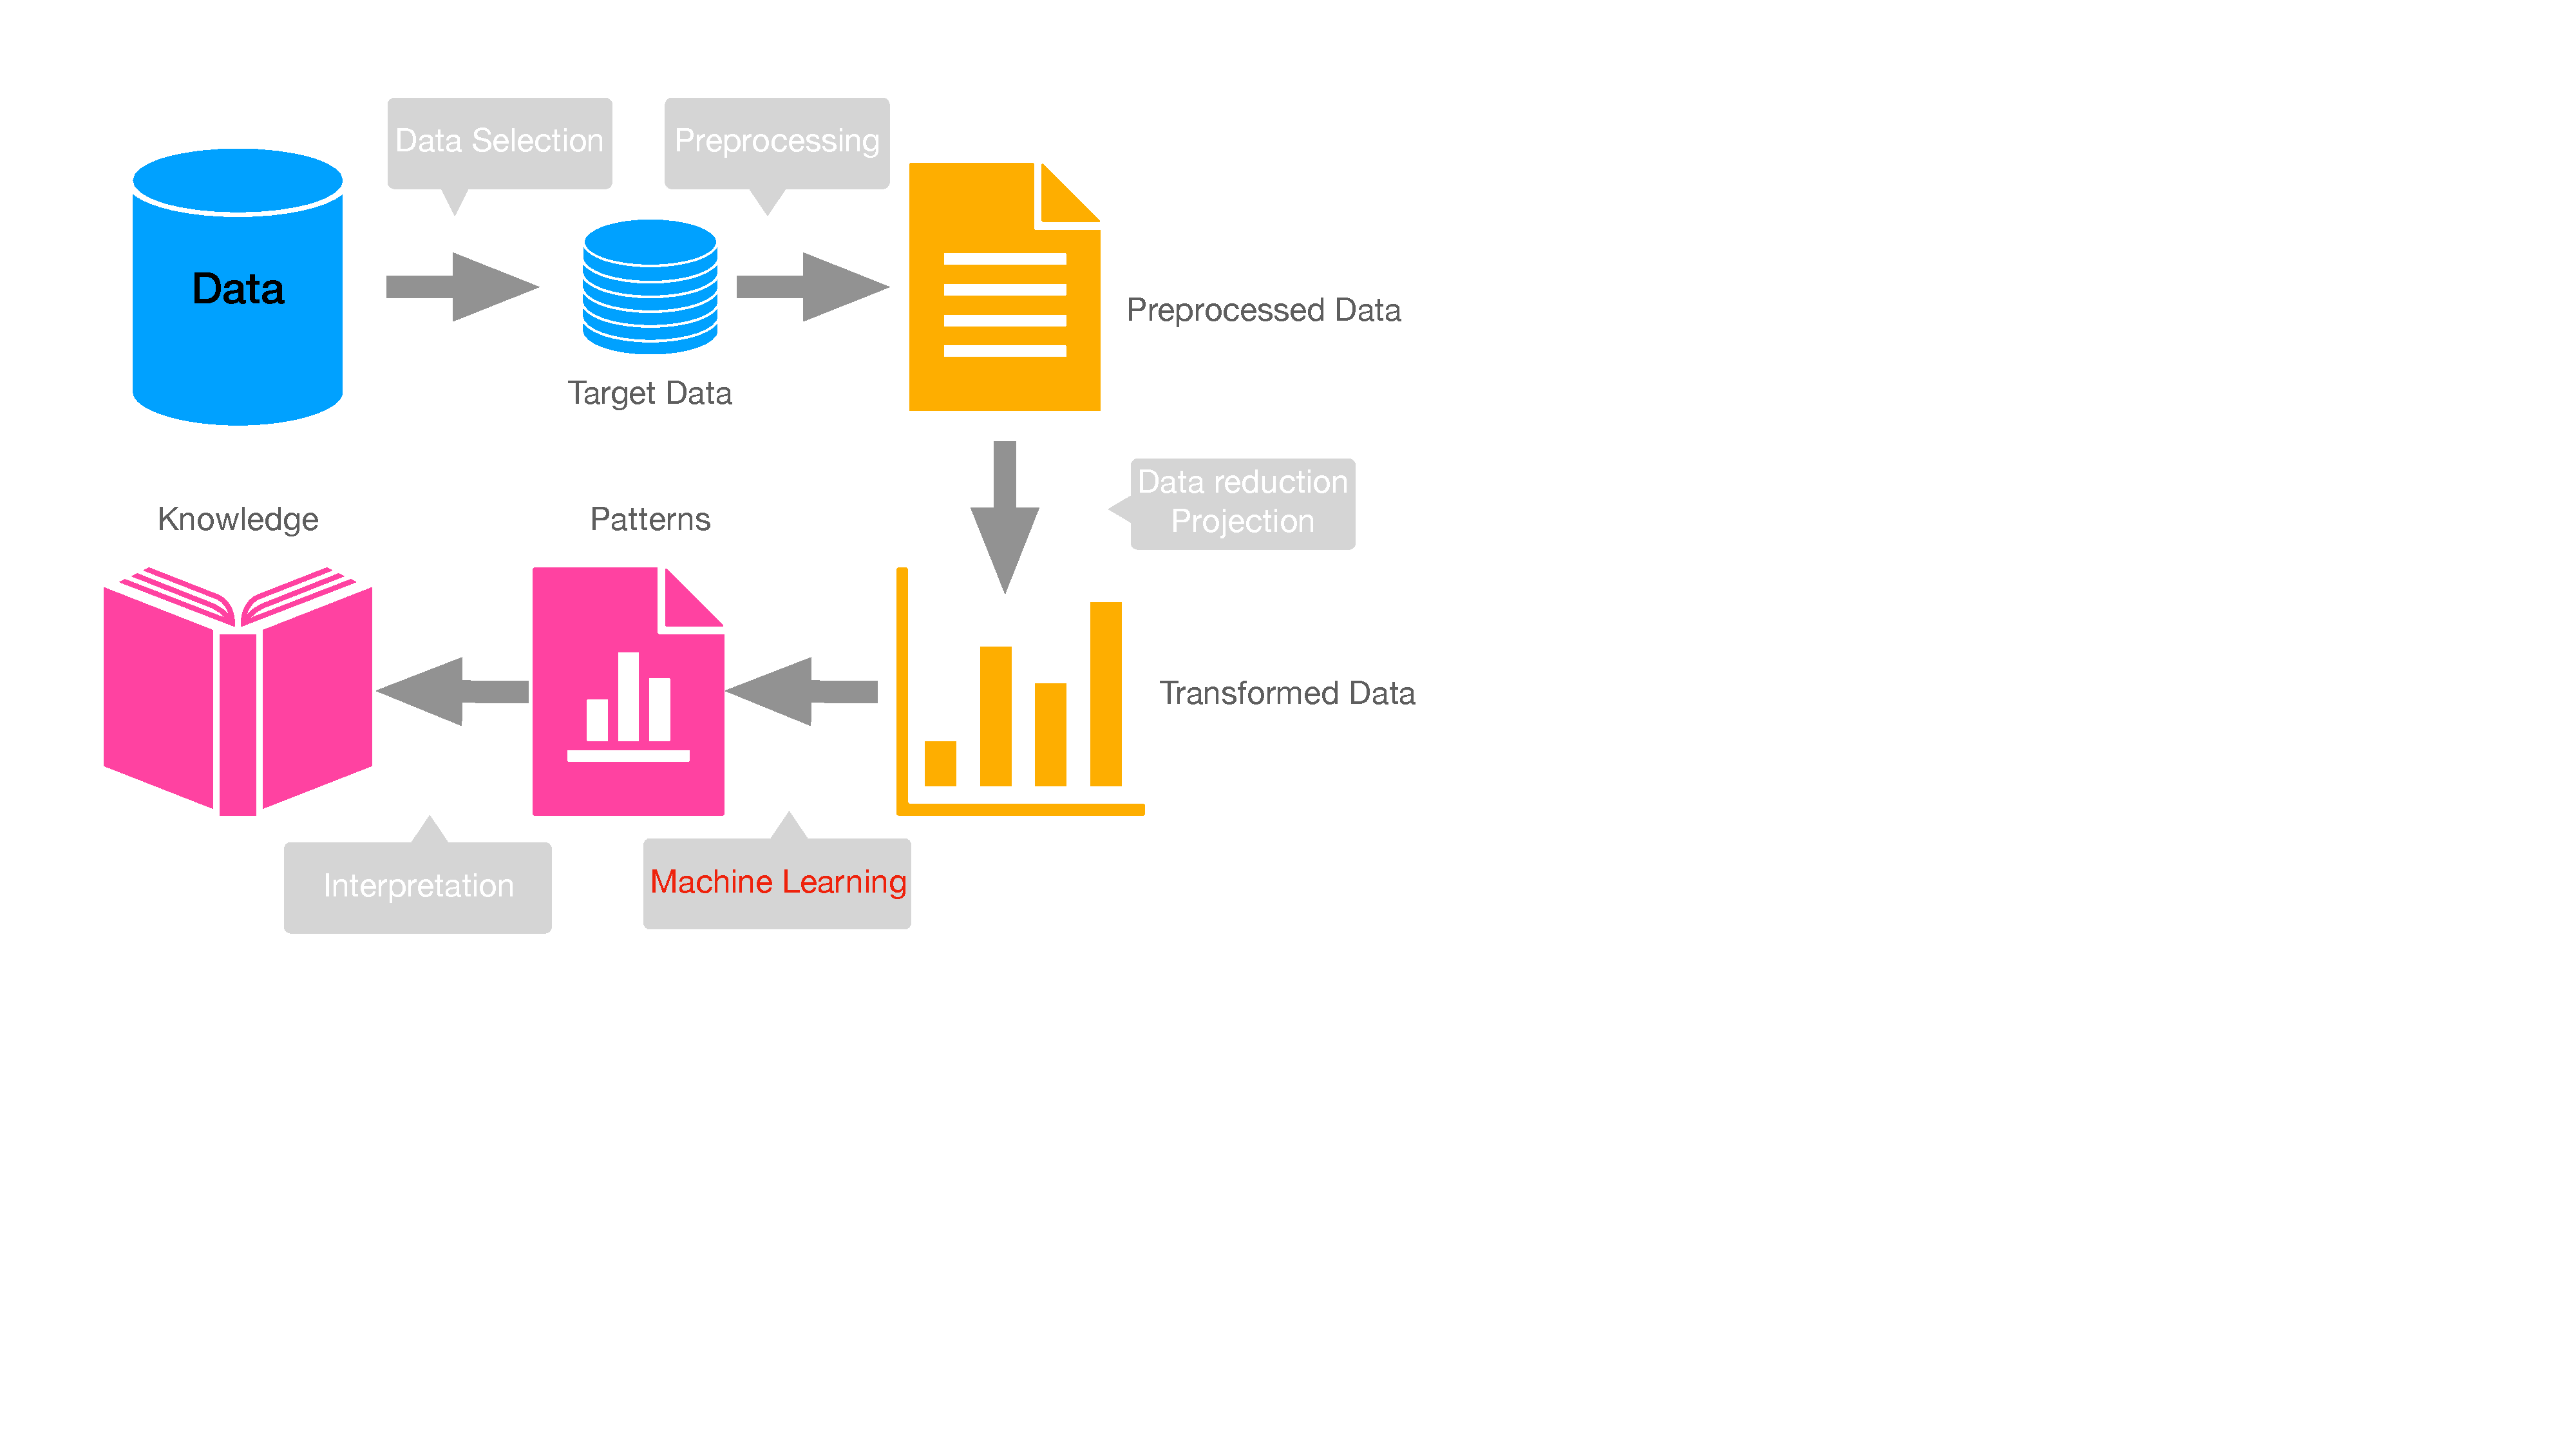
\includegraphics[width=1\textwidth]{graphics/KnowledgeDiscoveryProcess}

In a full data science process, \textcolor{magenta}{interpretability}
plays a key role in determining how to update the other steps of the
process for the next iteration. One interprets the results and tunes
the processing of the data, the loss function, the evaluation metric,
or anything else that is relevant, as shown in the diagram. \textcolor{magenta}{How
can one do this without understanding how the model works?}

\foilhead{Interpretability---5 principles}
\begin{description}
\item [{Principle-1}] An interpretable machine learning model obeys a domain-specific
set of constraints to allow it (or its predictions, or the data) to
be more easily understood by humans. These constraints can differ
dramatically depending on the domain.
\item [{Principle-2}] Despite common rhetoric, interpretable models do
not necessarily create or enable trust -- they could also enable
distrust. They simply allow users to decide whether to trust them.
In other words, they permit a decision of trust, rather than trust
itself.
\item [{Principle-3}] It is important not to assume that one needs to make
a sacrifice in accuracy in order to gain interpretability. In fact,
interpretability often begets accuracy, and not the reverse. Interpretability
versus accuracy is, in general, a false dichotomy in machine learning.
\item [{Principle-4}] As part of the full data science process, one should
expect both the performance metric and interpretability metric to
be iteratively refined. 
\item [{Principle-5}] For high stakes decisions, interpretable models should
be used if possible, rather than \textquotedblleft explained\textquotedblright{}
black box models.
\end{description}

\foilhead{Interpretability in the Knowledge Discovery Process}
\begin{itemize}
\item The knowledge discovery process in Figure 1 explicitly shows important
\textcolor{magenta}{feedback} loops. 
\item In practice, it is useful to create \textcolor{magenta}{many interpretable
models }(satisfying the known constraints) and have \textcolor{magenta}{domain
experts} choose between them. 
\begin{itemize}
\item Their rationale for choosing one model over another helps to refine
the definition of \textcolor{magenta}{interpretability}. 
\item Each problem can thus have its own \textcolor{magenta}{unique} interpretability
metrics (or set of metrics).
\end{itemize}
\end{itemize}

\foilhead{Interpretability Setup for Supervised Learning}
\begin{itemize}
\item Suppose we have
\begin{itemize}
\item data $\left\{ y_{i}\right\} _{i}$
\item models from a function class $\mathcal{F}$
\item a loss function $\mathcal{L}$
\end{itemize}
\item Then the \textcolor{magenta}{interpretable}, supervised learning process
can be defined as
\[
\min_{f\in\mathcal{F}}\frac{1}{n}\sum_{i}\mathcal{L}(f,y_{i})+\alpha P(f),
\]
where $P$ is an interpretability \textcolor{magenta}{penalty}, subject
to the interpretability \textcolor{magenta}{constraint},
\[
C(f)
\]
\item The loss function, as well as soft and hard interpretability constraints,
are chosen to \textcolor{magenta}{match} the context.
\item The goal of the \textcolor{magenta}{constraints} is to make the resulting
model $f$ or its predictions more interpretable: 
\begin{itemize}
\item The constraints would generally help us find models that would be
interpretable (if we design them well), and 
\item We might also be willing to consider slightly suboptimal solutions
to find a more useful model. 
\item The constant $\alpha$ trades off between accuracy and the interpretability
penalty, and can be tuned, either by cross-validation or by taking
into account the user\textquoteright s desired tradeoff between the
two terms.
\end{itemize}
\item Creating \textcolor{magenta}{interpretable} models can sometimes be
much more difficult than creating \textcolor{magenta}{black box} models
for many different reasons including: 
\begin{itemize}
\item (i) Solving the \textcolor{magenta}{optimization} problem may be computationally
hard, depending on the choice of constraints and the model class $\mathcal{F}.$ 
\item (ii) When one does create an interpretable model, one invariably realizes
that the \textcolor{magenta}{data} are problematic and require troubleshooting,
which slows down deployment (but leads to a better model).
\item (iii) It might not be initially clear which \textcolor{magenta}{definition}
of interpretability to use. This definition might require refinement,
sometimes over multiple iterations with domain experts.
\end{itemize}
\end{itemize}

\foilhead{Operational Interpretability}
\begin{itemize}
\item Define your \textcolor{magenta}{need}: 
\begin{itemize}
\item what your definition is and what you are optimizing
\item evaluate with your \textcolor{magenta}{end-task} in mind
\end{itemize}
\item The user/client does not need to undersatnd \textcolor{magenta}{every
single thing }about the model---all that is needed is knowing enough
for one's objectives.
\begin{itemize}
\item ``Enough'' is for what we are trying to do... and no more.
\end{itemize}
\end{itemize}

\foilhead{Interpretability is NOT}
\begin{itemize}
\item about making \textcolor{magenta}{ALL} models interpretable
\item about understading \textcolor{magenta}{EVERY SINGLE} line of a model
\item against developing \textcolor{magenta}{complex} models
\item only about gaining user \textcolor{magenta}{trust} and fairness...
\end{itemize}

\foilhead{Need for Interpretability}

We may \textcolor{magenta}{not }really need/want interpretabilty
\begin{itemize}
\item no significant \textcolor{magenta}{consequences}, or low stakes---eg.
advertising
\item \textcolor{magenta}{prediction} is what we care about
\item abundance of \textcolor{magenta}{empirical evidence} (logical/expected
reponse)
\item model is 100\% \textcolor{magenta}{reliable}
\item prevent users from \textcolor{magenta}{manipulating}/gaming the system
\end{itemize}
\begin{tcolorbox}[colback=red!5!white,colframe=red!75!black,title=Conclusion] 
We do not always need interpretability.
\end{tcolorbox}

\foilhead{Interpretability - Performance Trade-off}
\begin{itemize}
\item ``It is a \textcolor{magenta}{myth} that there is necessarily a trade-off
between accuracy and interpretability.'' {[}Rudin 2019{]} There is
no scientific evidence for this.
\item Carefully adding \textcolor{magenta}{structure} to the model---architecture,
prior, loss function---has long been done to improve performance
without interpretability in mind.
\end{itemize}
\begin{tcolorbox}[colback=red!5!white,colframe=red!75!black,title=Conclusion] 
An interpretability and performance trade-off often does not exist.  One should not equate interpretability with model sparsity.
\end{tcolorbox}

\foilhead{Interpretability and Trust?}
\begin{itemize}
\item Trust, fairness and interpretability are NOT the same thing...
\begin{itemize}
\item interpretability may improve them, but difficult to formalize
\item once formalized, you may not need interpretability...
\end{itemize}
\end{itemize}

\foilhead{Interpretability Methods}

\includegraphics[width=1\textwidth]{\string"graphics/decision tree COVID\string".png}
\begin{itemize}
\item Can you not just use \textcolor{magenta}{decision} trees?
\begin{itemize}
\item they can become very intricate and difficult to follow
\item they are not robust unless we use aggregation, but then we loose the
basic ``interpretabilty''
\end{itemize}
\end{itemize}
\begin{tcolorbox}[colback=red!5!white,colframe=red!75!black,title=Conclusion] 
Decision trees are not always interpretable---depends on your goal.
\end{tcolorbox}
\begin{itemize}
\item Other methods:
\begin{itemize}
\item linear classifiers
\item causality analysis
\end{itemize}
\end{itemize}

\foilhead{Types of Interpretability Methods}
\begin{itemize}
\item Explaining the data---EDA.
\item Building inherently interpretable models
\item Post-training intepretability methods
\end{itemize}
See work of {[}Doshi-Velez, Been Kim{]}

\foilhead{Explainable vs Interpretable}
\begin{itemize}
\item \textcolor{magenta}{Explainable AI} (XAI) attempts to explain a black
box using an approximation model, derivatives, variable importance
measures, or other statistics),
\item \textcolor{magenta}{Interpretable Machine Learning }is creating a
predictive model that is not a black box. 
\item Unfortunately, these topics are much too often lumped together within
the misleading term \textquotedblleft explainable artificial intelligence\textquotedblright{}
or \textquotedblleft XAI\textquotedblright{} despite a chasm separating
these two concepts. 
\item Explainability and interpretability techniques are not \textcolor{magenta}{alternative}
choices for many real problems; one of them (XAI) can be dangerous
for high-stakes decisions to a degree that the other is not.
\item \textcolor{magenta}{History}: Interpretable ML is not a subset of
XAI. The term XAI dates from \ensuremath{\sim}2016, and grew out of
work on function approximation; i.e., explaining a black box model
by approximating its predictions by a simpler model, or explaining
a black box using local approximations. Interpretable ML also has
a (separate) long and rich history, dating back to the days of expert
systems in the 1950\textquoteright s, and the early days of decision
trees. While these topics may sound similar they differ in ways that
are important in \textcolor{magenta}{practice}.
\end{itemize}
\begin{tcolorbox}[colback=red!5!white,colframe=red!75!black,title=Conclusions] 
When one explains black boxes, one expects to lose accuracy, whereas when one creates an inherently interpretable ML model, one does not. In fact, black boxes are generally unnecessary, given that their accuracy is generally not better than a well-designed interpretable model. 
\end{tcolorbox}

\foilhead{$\;$}

\vfill{}

\begin{center}
{\Large\textbf{\textcolor{blue}{DATA AND WORKFLOWS}}}{\Large\par}
\par\end{center}

\vfill{}


\foilhead{Trustworthy Data and Workflows}
\begin{itemize}
\item \textbf{Recall}: the complete Knowledge Discovery Process can impact
trustworthiness.
\item Understand your data source
\begin{itemize}
\item observational
\item simulated/synthetic
\item crowd-sourced
\end{itemize}
\item See above: how can AI go wrong?
\end{itemize}
\begin{tcolorbox}[colback=blue!5!white,colframe=blue!75!black,title=Note] 
AI in environmental applications takes a diverse set of data in the development and evaluation process. Building trust should start from accounting for the quality and limitations of these data sources.
\end{tcolorbox}

\foilhead{Observational Data}
\begin{itemize}
\item Environmental AI applications often rely on \textcolor{magenta}{in
situ observation data} to train or evaluate the model.
\begin{enumerate}
\item How representative (spatially and/or temporally) are these data? 
\item Are there any systematic bias/error of these data? 
\item What is the uncertainty of these data?
\end{enumerate}
\item \textcolor{magenta}{Satellite data }are another set of observational
data often used. You should consider:
\begin{itemize}
\item What is the quality of single-sensor data? 
\item How consistent are data from multiple sensors?
\item Is the satellite observation the same as what you want?
\end{itemize}
\end{itemize}

\foilhead{Simulated Data}

Why use simulated/synthetic data?
\begin{itemize}
\item Real data can be incomplete or inaccessible.
\begin{itemize}
\item Obtaining real data may be unethical---e cannot just infect people
to test a new vaccination strategy...
\end{itemize}
\item Real data cannot be directly used (due to restrictions such as privacy)
\item Common examples:
\begin{itemize}
\item Radiative transfer model simulation to simulate satellite data for
retrieval algorithm development
\item Reanalysis data (e.g., ERA-5)
\item Climate model simulations (e.g., CMIP6)
\item Large eddy simulation (LES)
\item Epidemiological projections (SIR)
\end{itemize}
\end{itemize}
Things to consider:
\begin{itemize}
\item There is an algorithm behind the simulated/synthetic data (including
input and output).
\item All of this must be trustwortty---see VV and UQ {[}Asch2022{]}
\end{itemize}

\foilhead{Crowd-Sourced Data}
\begin{itemize}
\item Crowd-sourced data provides unique opportunity to fill the data gap
in traditional data collection methods.
\item It is very challenging to establish consistent data quality for crowd-sourced
data...
\end{itemize}

\foilhead{Biases in Data}
\begin{itemize}
\item See above: how can AI go wrong?
\item \textcolor{magenta}{Non-representative} training data: rare events,
non-uniform sensors, remote areas not covered, phenomena not well-represented
at nigh, under-sampling
\item \textcolor{magenta}{Human-created} biases: 
\begin{itemize}
\item human labels can be wrong and the distribution discrete rather than
continuous, 
\item hail size is continuous yet people cluster labels to common objects
\end{itemize}
\item \textcolor{magenta}{Temporal or seasonal }biases
\item \textcolor{magenta}{Adversarial} data:
\begin{itemize}
\item crowd-sourced data can be hacked
\item false damage/storm/health reports
\item insurance fraud
\end{itemize}
\end{itemize}

\foilhead{Data Quality}
\begin{itemize}
\item Data \textcolor{magenta}{quality factors} to consider for YOUR use
cases:
\begin{itemize}
\item Bias/accuracy
\item Completeness/coverage
\item Resolution/frequency
\item Consistency
\item Timeliness
\end{itemize}
\item \textcolor{magenta}{Datasheets} or Data Management Plans (DMP)---``Documentation
to facilitate communication between dataset creators and consumers.\textquotedblright{}
\begin{itemize}
\item Motivation (why \& who created it)
\item Composition (what is in it)
\item Collection process (how it is created)
\item Preprocessing/cleaning/labeling (provenance)
\item Uses (intended \& not-suitable)
\item Distribution (who can use it)
\item Maintenance (dataset sustainability)
\end{itemize}
\item \textcolor{magenta}{Data Splitting} is indispensable for model training,
validation and testting
\begin{itemize}
\item spatial considerations: First Law of Geography (Tobler, 1970): everything
is related to everything else, but near things are more related than
distant things.
\begin{itemize}
\item Random split often ignores this \textcolor{magenta}{spatial} autocorrelation
aspect of the geospatial data and causes spillover effect. The result
can lead to decreased model performance in unseen situations.
\item Environmental data often have \textcolor{magenta}{temporal} autocorrelation
-- the data that from previous time periods are related to the current
time -- random splitting may not account for this information. Sometimes,
a chronological splitting can be more appropriate.
\end{itemize}
\item Imbalanced samples need to be dealt with caution to avoid the artificial
impact on the model performance.
\item Finally: \textcolor{red}{AVOID OVERFITTING}.
\end{itemize}
\end{itemize}

\foilhead{$\;$}

\vfill{}

\begin{center}
{\Large\textbf{\textcolor{blue}{COMMUNICATION}}}{\Large\par}
\par\end{center}

\vfill{}


\foilhead{UQ Methods}
\begin{enumerate}
\item Quantile regression (also works for ML models other than NNs)
\item CRPS loss function
\item Parametric prediction
\item Deep ensembles
\item Monte Carlo dropout 
\item Bayesian neural networks
\end{enumerate}
\begin{itemize}
\item Please consult
\begin{itemize}
\item {[}Asch2022{]}
\item blog: 
\end{itemize}
\end{itemize}
{\small\textcolor{blue}{\url{https://www.inovex.de/de/blog/uncertainty-quantification-deep-learning/}}}{\small\par}

\foilhead{Communicating Risk and Uncertainty}
\begin{itemize}
\item AI2ES Definition: Trust is the willingness to assume \textcolor{magenta}{risk}
by relying on or believing in the actions of another party.
\item How big the uncertainties are, matters in decision making!
\item Communicating \textcolor{magenta}{numerical risks}: 
\begin{itemize}
\item Use absolute risks (but also provide relative risks when dealing with
potential catastrophic events). 
\item For single unique events, use percent chance if possible, or if necessary,
\textquotedblleft 1 in X.\textquotedblright{} 
\item When appropriate, express chance as a proportion, a frequency, or
a percentage---it is crucial to be clear about the reference class.
\item Precision
\begin{itemize}
\item highest is a full, explicit probability distribution
\item lowest is explicit denial that uncertainty exists
\item inbetween, we have: distribution summaries, range or order-of-magnitude
assessment, qualifying verbal statement, list of possible scenarios,
informal mention of uncertainty
\end{itemize}
\end{itemize}
\end{itemize}
\begin{tcolorbox}[colback=green!5!white,  colframe=green!65!black,  title=Recommendations] 
\begin{enumerate}
  \item Communicating uncertainty can increase trust in the information, affect attitudes toward the messenger, and may sometimes delay decision making. 
  \item Align the format with the decision.
  \item And test your communications! 
\end{enumerate} 
\end{tcolorbox}

\foilhead{Graphics}
\begin{center}
\includegraphics[width=0.9\textwidth]{graphics/full-BAMS-D-21-0020\lyxdot 1-f1}
\par\end{center}

\begin{center}
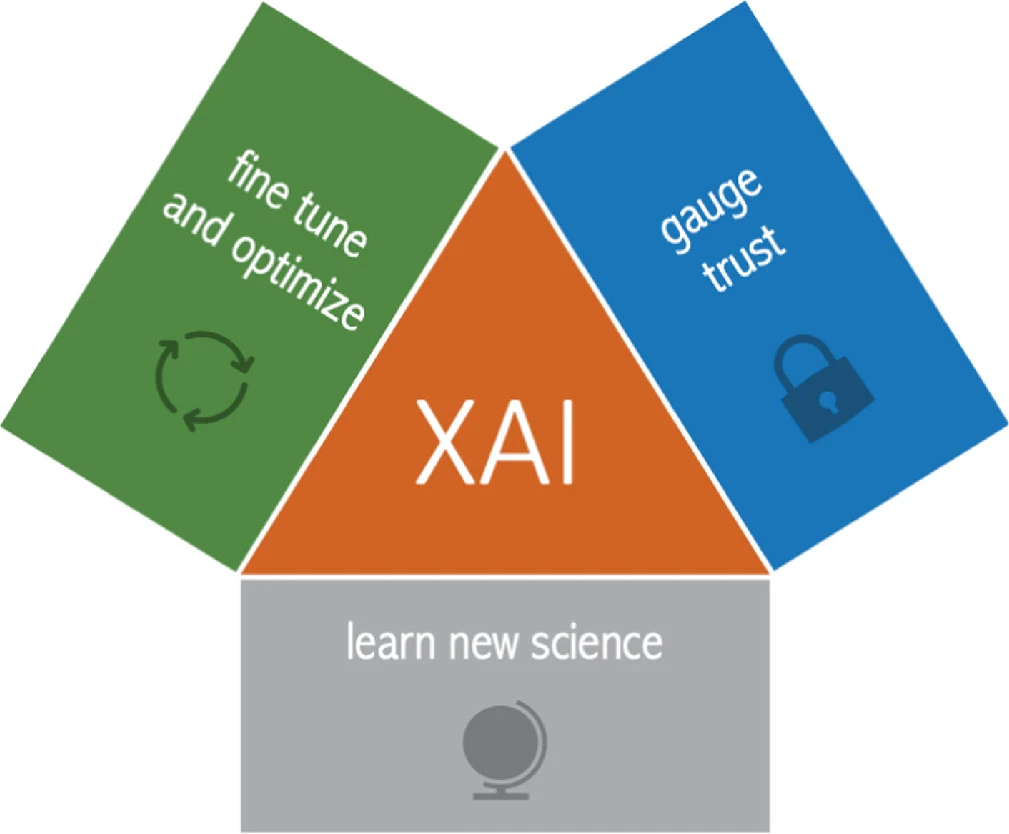
\includegraphics[width=0.75\textwidth]{graphics/XAI}
\par\end{center}

\foilhead{Bibliography}
\begin{thebibliography}{1}
\bibitem{Asch2022}M. Asch. \emph{Digital Twins: from Model-Based
to Data-Driven.} SIAM, 2022.

\bibitem{XAI}A. Holzinger, et al. (editors).\emph{ xxAI - Beyond
Explainable AI}. Springer. 2022

\bibitem{BAMS}McGovern, A., Gagne, D.J., Wirz, C.D., Ebert-Uphoff,
I., Bostrom, A., Rao, Y., Schumacher, A., Flora, M., Chase, R., Mamalakis,
A. and McGraw, M. (2023) \emph{Trustworthy Artificial Intelligence
for Environmental Sciences: An Innovative Approach for Summer School.}
Bulletin of the American Meteorological Society, Apr 2023. 

\bibitem{EDS}McGovern, Amy, Imme Ebert-Uphoff, David John Gagne II
and Ann Bostrom (2022) \emph{Why we need to focus on developing ethical,
responsible, and trustworthy artificial intelligence approaches for
environmental science}, Environmental Data Science, 1, E6. 

\bibitem{BAMS2}McGovern, A., and Coauthors, 2022: \emph{NSF AI Institute
for Research on Trustworthy AI in Weather, Climate, and Coastal Oceanography
(AI2ES)}. Bull. Amer. Meteor. Soc., 103, E1658--E1668

\bibitem{Rudin}C. Rudin. C. Chen. Z Chen. H Huang. L Semenova. C
Zhong. \textquotedbl Interpretable machine learning: Fundamental
principles and 10 grand challenges.\textquotedbl{} Statistics Surveys,
16 1 - 85, 2022. https://doi.org/10.1214/21-SS133.

\end{thebibliography}

\end{document}
